%%%%%%%%%%%%%%%%%%%%%%%%%%%%%%%%%%%%%%
% LaTeX poster template
% Created by Nathaniel Johnston
% August 2009
% http://www.nathanieljohnston.com/index.php/2009/08/latex-poster-template/
%%%%%%%%%%%%%%%%%%%%%%%%%%%%%%%%%%%%%%

\documentclass[final]{beamer}
\usepackage[size=custom, width=116.84, height=101.6, scale=0.85]{beamerposter}
\usepackage{graphicx}			% allows us to import images
\usepackage{subfig}
%\setbeamertemplate{caption}[numbered]

%-----------------------------------------------------------
% Define the column width and poster size
% To set effective sepwid, onecolwid and twocolwid values, first choose how many columns you want and how much separation you want between columns
% The separation I chose is 0.024 and I want 4 columns
% Then set onecolwid to be (1-(4+1)*0.024)/4 = 0.22
% Set twocolwid to be 2*onecolwid + sepwid = 0.464
%-----------------------------------------------------------

\newlength{\sepwid}
\newlength{\onecolwid}
\newlength{\twocolwid}
\newlength{\threecolwid}
\setlength{\sepwid}{0.021739130434782608\paperwidth}
\setlength{\onecolwid}{0.30434782608695654\paperwidth}
\setlength{\twocolwid}{0.63043478260869568\paperwidth}
\setlength{\threecolwid}{0.95652173913043481\paperwidth}
\setlength{\topmargin}{-0.5in}
\usetheme{confposter}

%-----------------------------------------------------------
% Define colours (see beamerthemeconfposter.sty to change these colour definitions)
%-----------------------------------------------------------

\setbeamercolor{block title}{fg=ucdblue,bg=white}
\setbeamercolor{block body}{fg=black,bg=white}
\setbeamercolor{block alerted title}{fg=white,bg=ucdblue}
\setbeamercolor{block alerted body}{fg=black,bg=ucdblue!10}

%-----------------------------------------------------------
% Name and authors of poster/paper/research
%-----------------------------------------------------------

\title{Human Control of Bicycle Dynamics with Experimental Validation\\
and Implications for Bike Handling and Design}

\author{Mont Hubbard, Ronald A. Hess, Dale L. Peterson, Jason K. Moore}

\institute
{
\centering
\begin{tabular}{c}
Department of Mechanical and Aerospace Engineering, University of California, Davis\\
\small{NSF Grant \# 0928339, NSF Program Name: Civil, Mechanical and Manufacturing Innovation}
\end{tabular}
}
%-----------------------------------------------------------
% Start the poster itself
%-----------------------------------------------------------
% The \rmfamily command is used frequently throughout the poster to force a serif font to be used for the body text
% Serif font is better for small text, sans-serif font is better for headers (for readability reasons)
%-----------------------------------------------------------

\begin{document}
\frame{

\begin{center}
% Divide the frame into columns
\begin{columns}[t] % the [t] option aligns the column's content at the top

% Space column
\begin{column}{\sepwid}\end{column}	% empty spacer column

% First column
\begin{column}{\onecolwid}

  \begin{block}{Introduction}
    \rmfamily{

    This poster presents interim results of the project whose overall research
    objective is to develop experimentally validated dynamic models of bicycles
    controlled by human riders.  In the first half of the project we
    accomplished four goals: 1) studied analytically steady turning behavior of
    the bicycle; 2) built and tested two experimental bicycles to identify
    human control laws and to validate the analytic bicycle models; 3) measured
    parameters of a family of bicycles; 4) developed preliminary theoretical
    models for human rider control laws based on previous aircraft-based
    human-operator models.  If successful, this research will improve the
    fundamental understanding of how humans interact with bicycles and will aid
    in design of bicycles for wider populations and for a wider range of tasks.

    Voluminous research over the last hundred years has resulted in no useful
    design guidelines for the construction of bicycles with desired handling
    qualities.  Even the simplest models with a rigidly attached rider have yet
    to be completely understood. Deeper questions regarding the fundamental
    control methods and objectives of a human rider~\cite{Hess1987a} also
    remain unanswered and are the key to understanding handling. Our research
    is designed to answer some of these questions.

    Bicycle stability has been studied for more than a
    century~\cite{Whipple1899} , but only recently have researchers agreed on
    the stability, dynamic response, and characteristics of the simplest
    bicycle models, constrained to constant velocity linear and circular
    motions~\cite{Meijaard2007, Basu-Mandal2007}. Several researchers have also
    successfully developed control algorithms capable of stabilizing a bicycle
    (both theoretically and in practice) with various inputs such as steering
    torque~\cite{Fajans2000}, rider lean~\cite{Zytveld1975}, and gyroscopic
    stabilization~\cite{Gallaspy2000}. Much less is understood about the added
    complexity that including a rider brings to the problem and, in
    particular, the identification of control strategies that a human might
    employ.  Few studies have touched on these issues~\cite{Roland1972,
    Lunteren1970b}.

    Designers of manually controlled vehicles have consistently sought
    correlations between the vehicle configuration, task performance and ease
    of control, or ``handling qualities.'' Aircraft flight control has research
    dating from the mid-1950's~\cite{Anon1954}. In aircraft applications,
    handling qualities refer to those characteristics that determine the ease
    and precision with which a pilot may complete a given
    task~\cite{Cooper1969}. There are two reasons why bicycle manual control
    and handling qualities are important.  First, the bicycle represents a
    challenging manual control problem, the study of which can illuminate human
    control in general. Second, deeper understanding of human interaction with
    bicycles can lead to improved designs that handle better at low speeds
    favored by the elderly, disabled, and children or that handle better with
    large cargo loads.

  }
  \end{block}

  \begin{block}{Steady Turning}
    \rmfamily{

    The upright zero-steer configuration of an uncontrolled laterally symmetric
    bicycle is an equilibrium configuration at any speed, making speed a
    natural choice to parameterize. All other dynamic equilibrium
    configurations (i.e. non-zero lean or steer) permit only a single speed
    (forward or backward). Thus, stability of steady turns must be visualized
    using at least two parameters; we choose the lean and steer angles.  At
    each lean-steer configuration we compute the dynamic equilibrium (steady
    turning) speed, required steer torque, wheel contact forces, and the
    stability of this dynamic equilibrium point. The results of these
    calculations are presented as level curves (in the lean-steer plane) of
    speed, steer torque, and required tire friction coefficients.  Regions in
    the lean-steer plane where the turns are stable are also shown, and whether
    the dominant eigenvalue is real or complex.

    Five solid black curves are shown on both plots of Figure 1. On the far
    left and right of each plot, these black curves denote the minimum and
    maximum lean angles obtainable, regardless of the dynamics. The next two
    black curves form the larger two triangular shaped regions in the lower
    right and upper left regions of each plot. The first of these, the nearly
    vertical curve, characterizes static equilibrium configurations. The second
    corresponds to the infinite speed or zero-gravity steady turning solution. The final solid
    black curve contained within the triangular regions is the zero level curve
    for rear wheel normal force. Realistic steady turns must lie between this curve and the static
    equilibrium curve.

    \begin{figure}[h]
      \begin{center}

        \subfloat[Level curves of steer torque shown with green curves. Stable
        regions are highlighted with solid green and solid red. Solid green
        corresponds to stable eigenvalues for which the dominant (nearest the
        j-$\omega$ axis) eigenvalue is complex; solid red corresponds to stable
        eigenvalues for which the dominant eigenvalue is real.
        ]{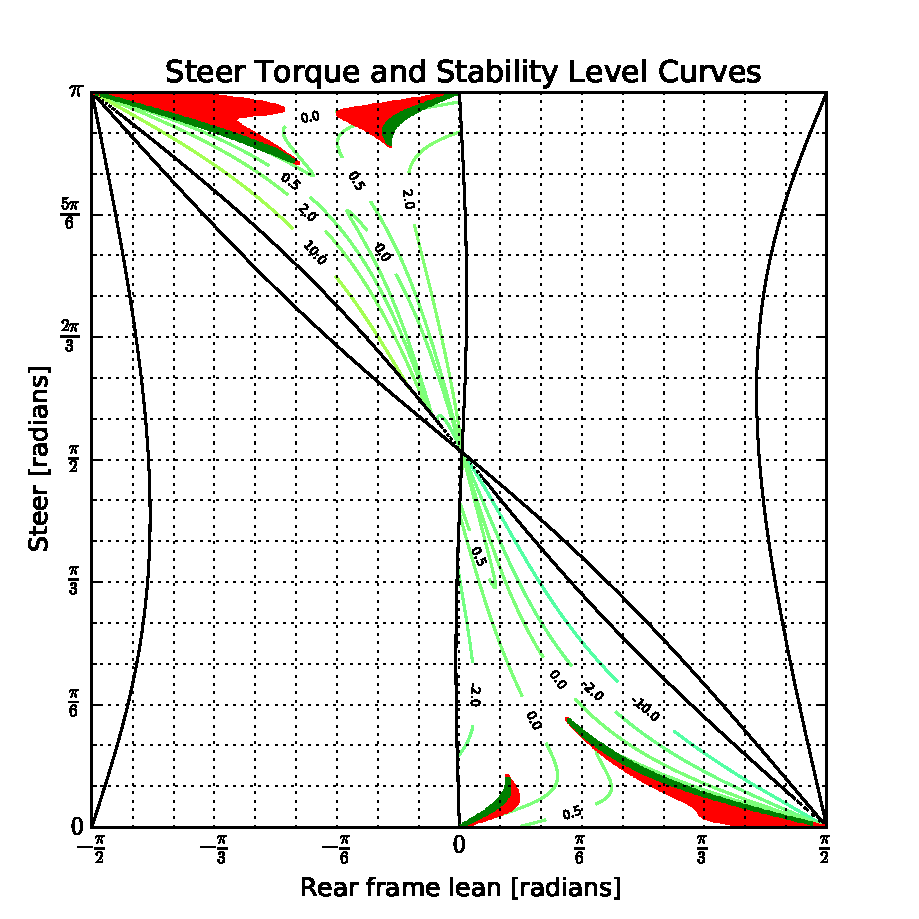
\includegraphics{steady_benchmark_tau_stable.pdf}}\quad
        \subfloat[Curves of constant velocity and required tire friction
        coefficient. Velocity level curves emanate from the origin and also
        pass through the point near lean=0, steer=$\pi$/2. Friction
        coefficient level curves emanate from the steer=0 axis, pass through
        the point near lean=0, steer=$\pi$/2, and then continue to the
        steer=$\pi$ axis. These emanating curves are explained by the fact that
        the upright (zero lean and steer) is an equilibrium for all speeds.
        Dashed friction curves correspond to the front wheel, solid correspond
        to the rear wheel. For a fixed steer, as lean (and hence velocity) is
        increased, these dashed curves will be reached first, indicating that a
        higher front wheel friction coefficient is desirable to prevent front
        wheel slip.]{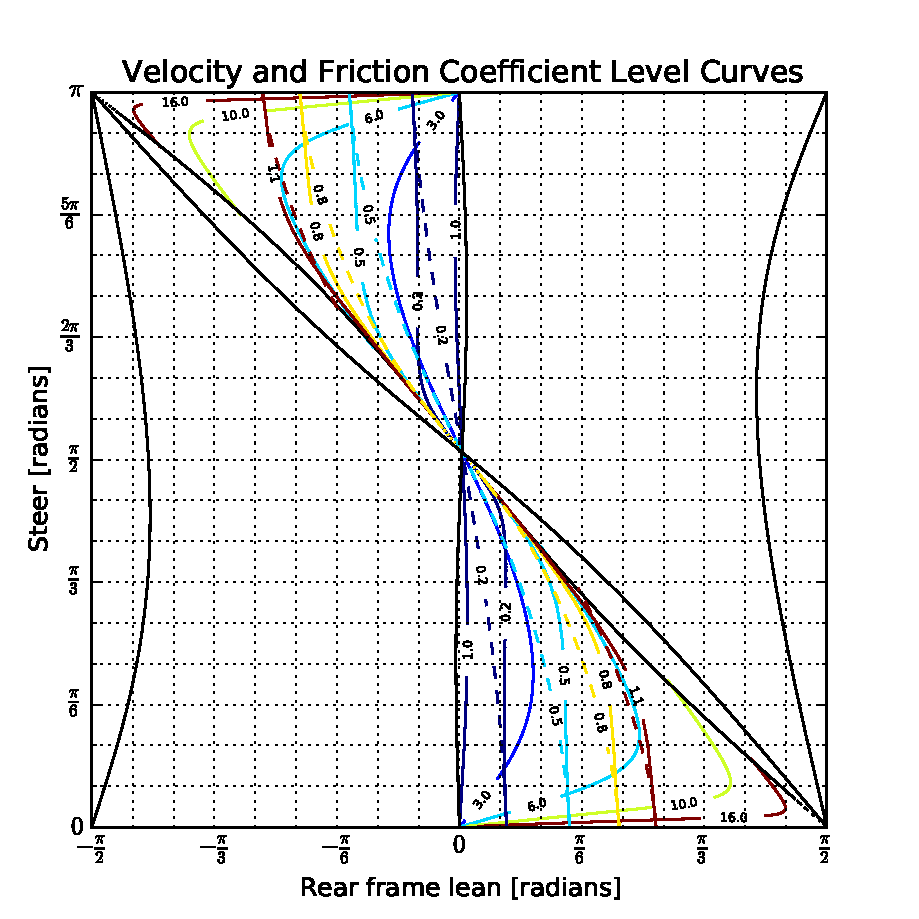
\includegraphics{steady_benchmark_vmew.pdf}}

        \caption{\rmfamily{(1)}}
      \end{center}
    \end{figure}
  }
  \end{block}

\end{column}

% Spacer column
\begin{column}{\sepwid}\end{column} % empty spacer column

% Second column
\begin{column}{\onecolwid}

  \begin{block}{Experimental bicycles}
    \rmfamily{
    We have developed two bicycles for validating our bicycle dynamics and
    human control models Fig.~\ref{fig:Bicycles}. The first
    Fig~\ref{fig:RobotBicycle} is instrumented with sensors for measuring the
    dynamics of the bicycle and is capable of steering and balancing on its
    own. It will be used to validate the non-linear model
    typically used for bicycle dynamics studies~\cite{Meijaard2007} and to test
    various control algorithms. These will allow us to verify response of the
    closed loop system to various types of inputs. System identification
    techniques will be used with experimentally measured dynamic
    responses. These experiments will lead to a quantitative description of how
    well a rigid body model, which ignores tire dynamics, can be used to
    describe the motion of real bicycles. The second
    Fig.~\ref{fig:InstrumentedBicycle} is an instrumented bicycle that will be
    controlled by a human rider. It has two configurations; one that rigidifies
    the rider and one that allows for some rider upper-body flexibility. The
    instrumentation is capable of measuring bicycle and rider kinematics along
    with the forces between the rider and vehicle by means of force transducers at
    the steering column, seat post and foot pegs. The rider will execute
    maneuvers on both a treadmill and a smooth indoor floor. The experimental
    results will be used to validate our human control hypotheses.
    }
    \begin{figure}[h]
      \begin{center}
        \subfloat[]{\label{fig:RobotBicycle}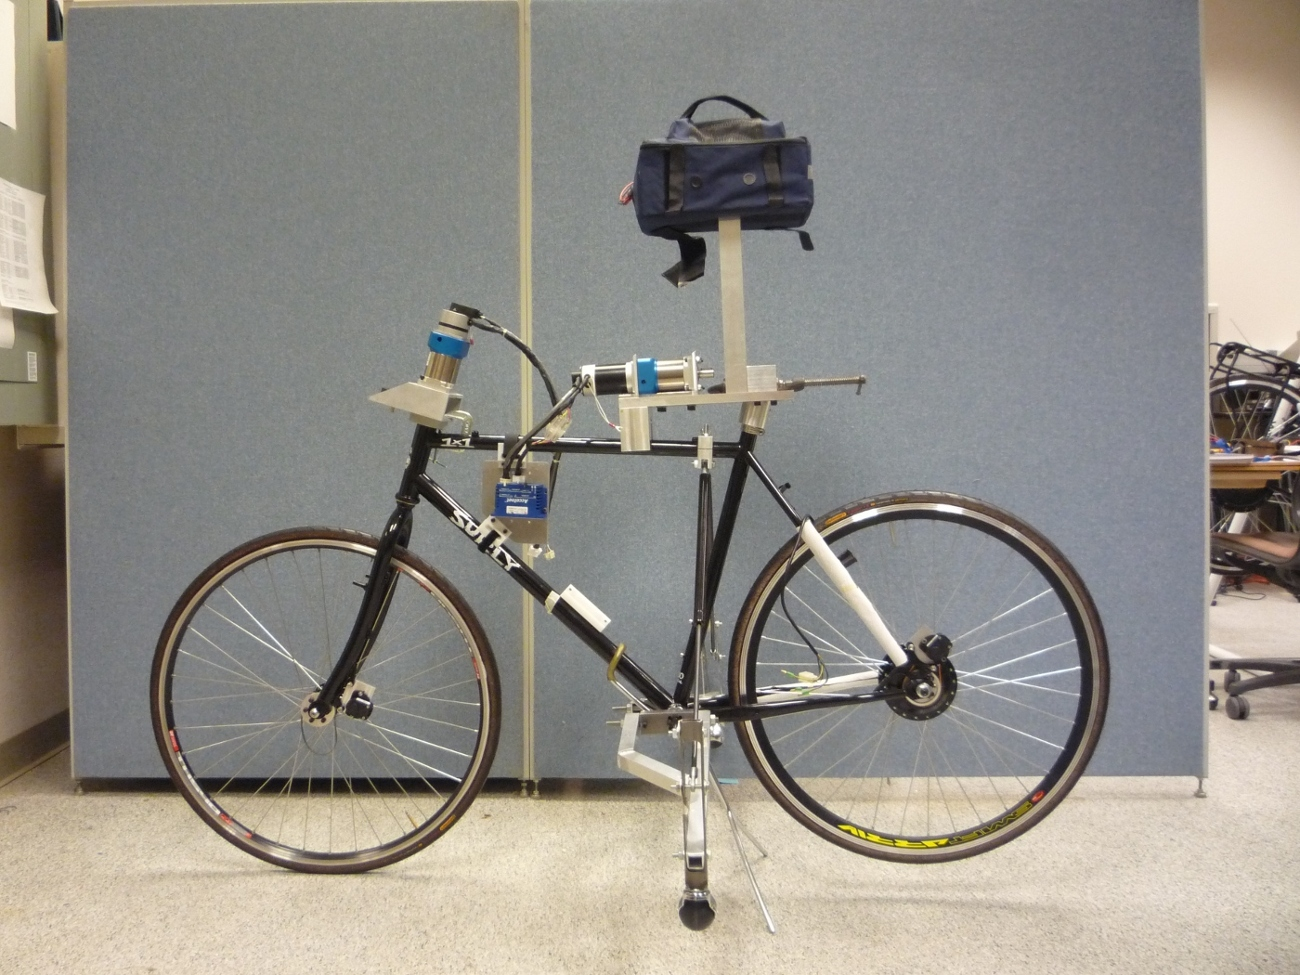
\includegraphics{RobotBicycle.jpg}}
        \qquad
        \subfloat[]{\label{fig:InstrumentedBicycle}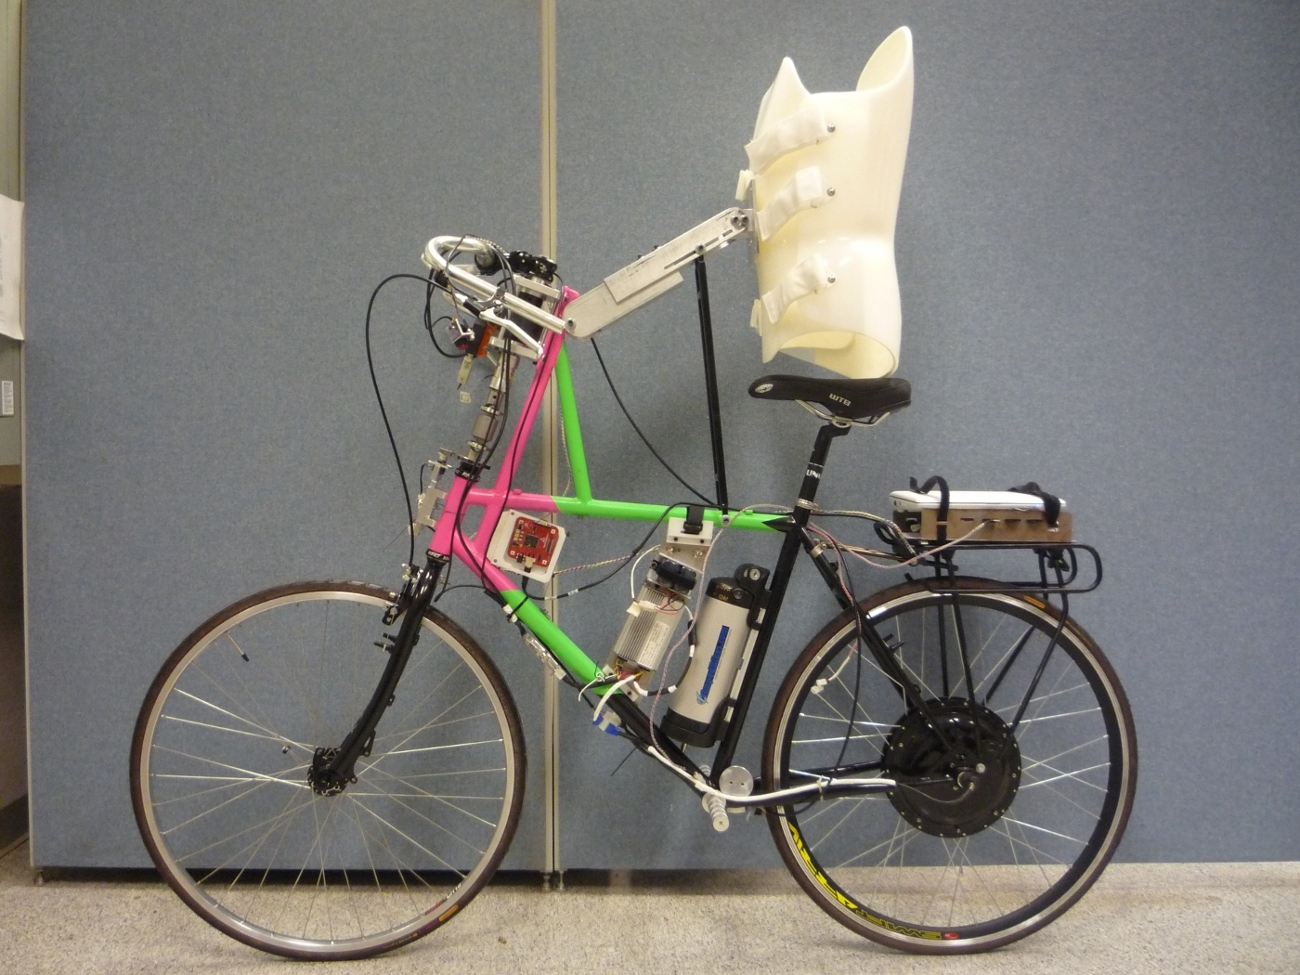
\includegraphics{InstrumentedBicycle.jpg}}
        \caption{\rmfamily{(2)\quad(a) The robotic bicycle complete with steer, rider lean, and
        wheel speed motors and controllers. (b) The instrumented bicycle with
        hub motor, inertial measurement unit, force transducers and a body cast
        to rigidify the rider.}}
        \label{fig:Bicycles}
      \end{center}
    \end{figure}
  \end{block}

  \begin{block}{Parametric descriptions of a family of bicycles}
    \rmfamily{
    Accurate measurements of a bicycle's physical parameters are required for
    realistic dynamic simulations and analysis. The most basic models require
    the geometry, mass, mass location and mass distributions of the rigid
    bodies. We have developed an accurate technique to measure the
    bicycle parameters required for the benchmark Whipple bicycle model
    presented in~\cite{Meijaard2007}. This model is composed of four rigid
    bodies, has ideal rolling and frictionless joints, and is laterally
    symmetric. A set of 25 parameters can be used to describe the geometry,
    mass, mass location and mass distribution of each of the bicycles' primary
    rigid bodies. The experimental methods used to estimate the parameters are
    similar to those in \cite{Kooijman2006} but have been refined for improved
    accuracy and methodology. We measured the physical characteristics of six
    different bicycles, two of which were set up in two different
    configurations for a total of eight parameter sets. The six bicycles,
    chosen for both variety and convenience, are as follows: Batavus Browser, a
    Dutch style city bicycle measured with and without instrumentation; Batavus
    Stratos Deluxe, a Dutch style sporty city bicycle; Batavus Crescendo Deluxe
    a Dutch style city bicycle with a suspended fork; Gary Fisher Mountain
    Bike, a hardtail mountain bicycle; Bianchi Pista, a modern steel frame
    track racing bicycle; and Yellow Bicycle, a stripped down aluminum frame
    road bicycle measured in two configurations, the second with the fork
    rotated in the headtube 180 degrees for larger trail. We calculated both
    the parameter sets and linear model coefficient matrices for the bicycles
    alone and the bicycles with the same rigid rider for all eight bicycles. In
    addition, the uncertainties in the parameters and matrix coefficients, are
    included for the bicycle without the rider. Figure~\ref{fig:Eig}
    shows an example of how the parameter sets may be used to compare the
    linear dynamics of a bicycle.  Furthermore, the parameter sets were used in
    our closed loop system design and handling quality metrics described
    hereafter.
    }
    \begin{figure}[h]
      \begin{center}
        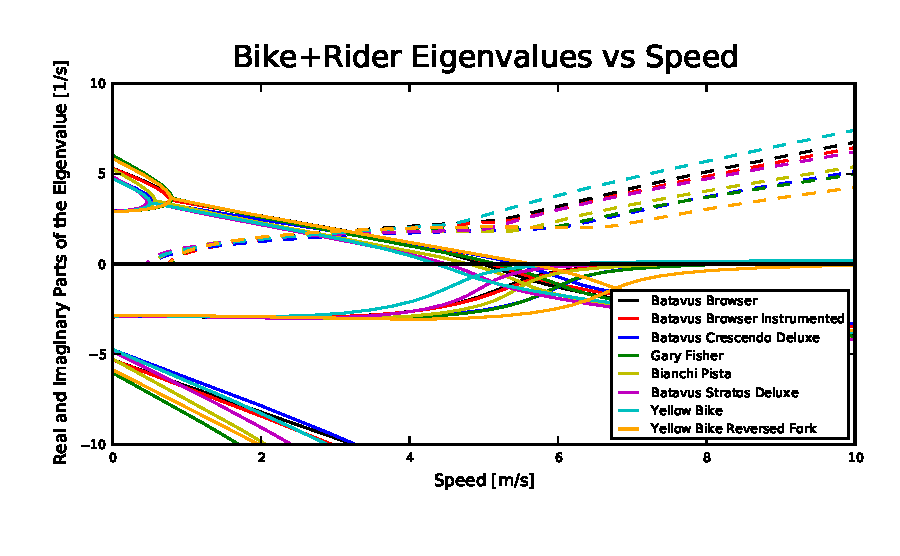
\includegraphics[width=12in]{eig_plot.pdf}
        \caption{\rmfamily{(3)\quad The eigenvalues versus speed for eight different bicycles with
        the same rigid rider.  The open loop eigenvalues can predict
        uncontrolled stability and may have correlation to handling. For
        example, the plot shows that the stable speed range can vary greatly
        between bicycles.}}
      \label{fig:Eig}
      \end{center}
    \end{figure}
  \end{block}

\end{column}

% Spacer column
\begin{column}{\sepwid}\end{column} % empty spacer column

% The third column
\begin{column}{\onecolwid}

  \begin{block}{Human Control Model}
    \rmfamily{
    \emph{Linear Bicycle Model:} A complete description of the development of
    the linear bicycle and rider control models can be found
    in~\cite{Hess1990}. The resulting equations of motion are two coupled,
    second-order ode's for the lean $\phi$ and steer $\delta$ variables with
    steering torque and lean torque as inputs and gravity and speed as
    parameters.

    \emph{Rider Control Model:} We assume the rider can sense the five
    variables: steer angle $\delta$, lean angle $\phi$ and rate $\dot{\phi}$,
    yaw angle $\psi$ and lateral deviation $y$, both as deviations from a
    desired reference line. The feedback structure differs from that described
    in reference \cite{Hess2006} by the appearance of an additional, inner loop
    featuring feedback of steering angle through a gain $K_\phi$ to a form of
    the neuromuscular transfer function $G_{nm}$ modified from \cite{Hess2006}.
    The addition of the $\delta$ feedback loop as well as the higher-bandwidth
    of $G_{nm}$ compared with those in \cite{Hess2006} are required to obtain
    closed-loop rider/vehicle dynamics with bandwidths sufficient to stabilize
    the bicycle across the velocity ranges considered. This loop includes
    ``force/feel system'' dynamics excluded in reference \cite{Hess2006}. See
    also \cite{Hess1997a} and \cite{Hess1990}. Only three gains, $K_\delta$,
    $K_\phi$ , and $K_{\dot{\phi}}$ are required to parameterize the rider
    balancing model.

    \begin{figure}[h]
      \begin{center}
        \subfloat[]{\label{fig:BalanceLoop}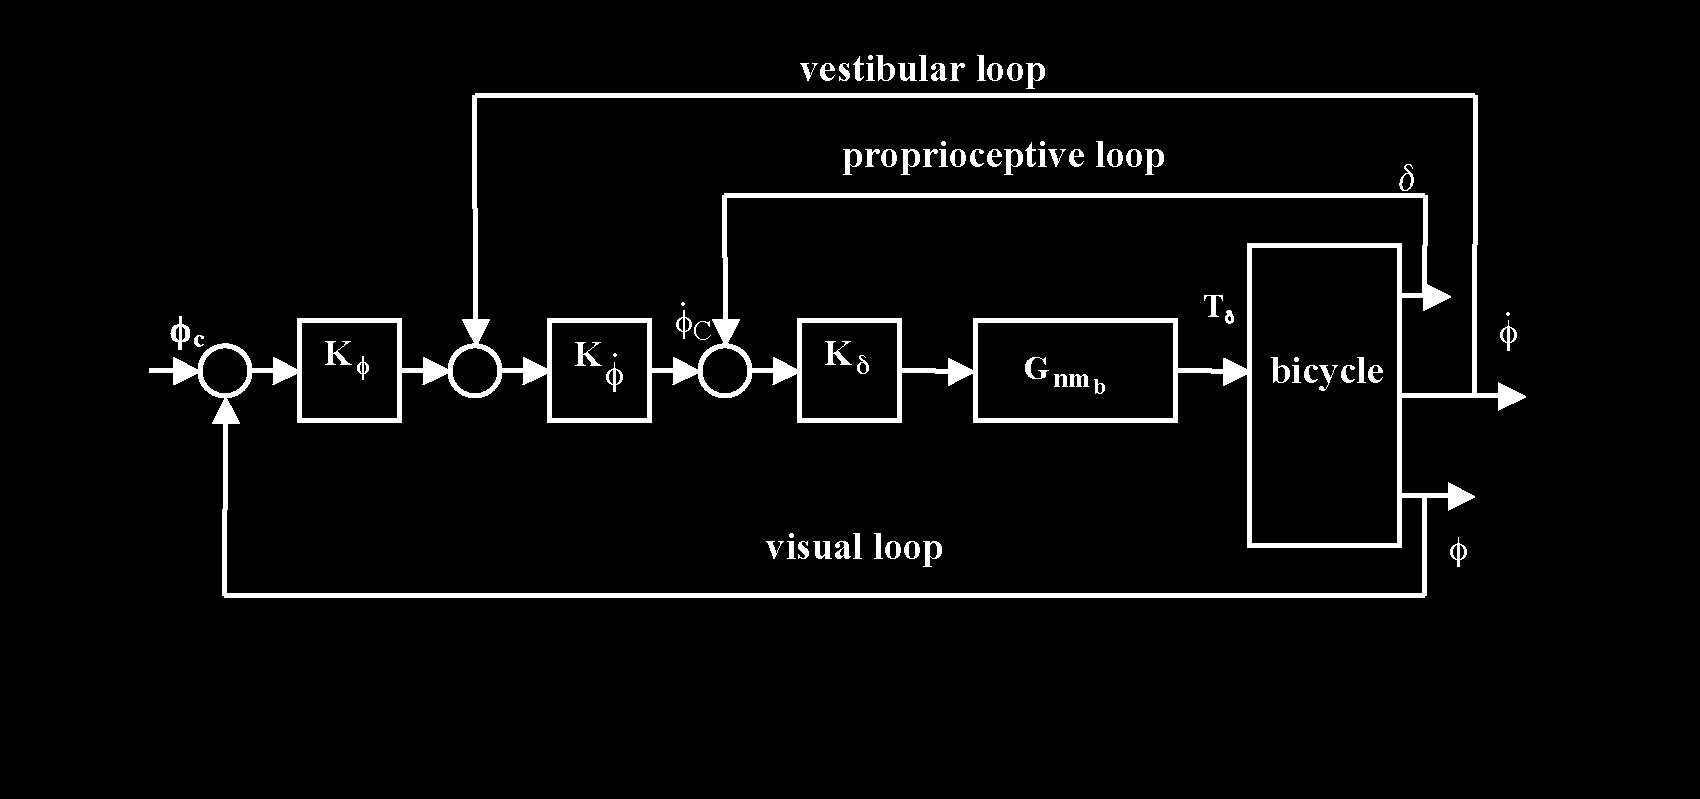
\includegraphics[width=6.5in]{Fig6.jpg}}
        \quad
        \subfloat[]{\label{fig:FeedbackLoop}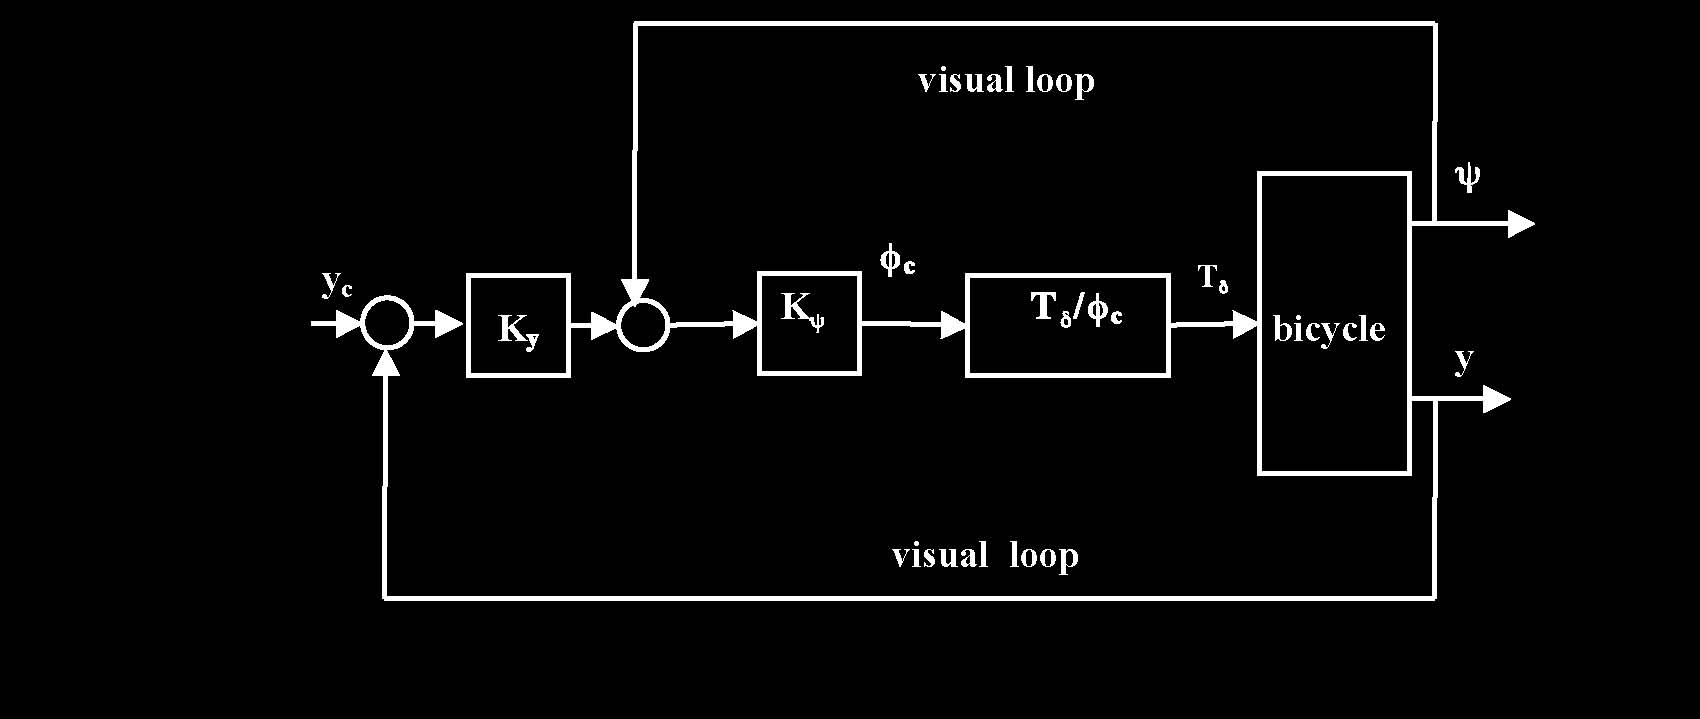
\includegraphics[width=6.5in]{Fig7.jpg}}
        \caption{\rmfamily{(4)\quad(a) Schematic of inner ``balance'' control
        loops. (b) Complete rider/vehicle feedback model.}}
      \end{center}
      \label{fig:Loops}
    \end{figure}
    The model does not include elaborate preview models. Nevertheless, the most
    likely sensory feedback modalities are included in
    Fig.~\ref{fig:BalanceLoop}, i.e. feedback from the proprioceptors in the
    rider's arms (muscle spindles and joint angle receptors), feedback from the
    vestibular sensors in the inner-ear (the semi-circular canals), and
    feedback from the visual system. Models of the sensory systems have not
    been included. The complete rider/vehicle model, including two outer-loop
    closures using two feedback gains $K_\psi$, and $K_y$ for heading $\psi$
    and lateral deviation from a desired path $y$, is shown in
    Fig.~\ref{fig:FeedbackLoop}.  The five control gains are determined using
    frequency response techniques for successive loop closure (beginning with
    the innermost loop and working out) and the ``crossover model'' as
    described in \cite{Hess1990}.

    Figure~\ref{fig:TimeHistory} shows the steering angles and closed loop
    performance of the hypothesized human controller during a double lane
    change maneuver for a nominal set of feedback gains chosen in the above
    manner for the population of 8 bicycles described above. Although all 8
    bicycles have similar dynamic characteristics, some differences are
    apparent.  Non-minimum phase closed loop behavior is evident.
    \begin{figure}[h]
      \begin{center}
        \subfloat[]{\label{fig:TimeHistory}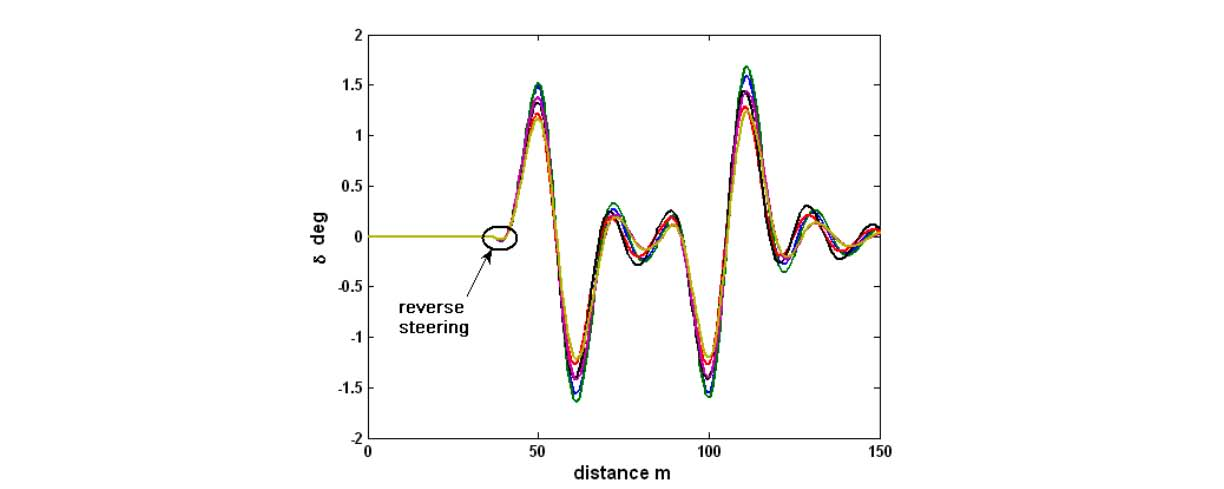
\includegraphics[width=6.5in]{Fig28.jpg}}
        \qquad
        \subfloat[]{\label{fig:Handling}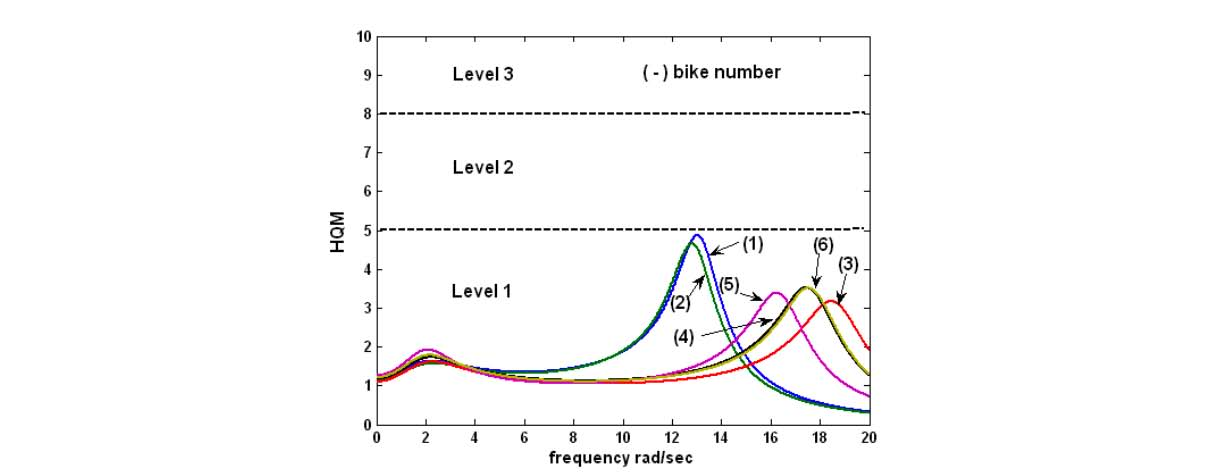
\includegraphics[width=6.5in]{Fig19.jpg}}
        \caption{\rmfamily{(5)\quad(a) Steering angles in double lane change maneuver.  (b)
        Handling Quality Metrics for six of the bicycles above.}}
      \end{center}
      \label{fig:TimeHandling}
    \end{figure}

    Although not described here, one of the features of the human operator
    control proposed in \cite{Hess1990} is that it is possible to identify
    Handling Quality Metrics from certain characteristics of closed loop
    transfer function frequency responses. These metrics predict the handling
    level (1, 2 or 3) corresponding to the Cooper-Harper \cite{Cooper1969}
    scale commonly used in rating handling qualities for aircraft.
    Fig.~\ref{fig:Handling} shows the resulting Handling Quality Metrics for
    six of the eight bicycles mentioned above, indicating Level 1 (desired)
    task-independent handling qualities at the speed in question (7.5 m/sec).
    }
  \end{block}

  % References
  \begin{block}{References}
    \tiny{\rmfamily{
    \bibliographystyle{ieeetr}
    \bibliography{bicycle}
    }}
  \end{block}

\end{column}

% Last spacer column
\begin{column}{\sepwid}\end{column}			% empty spacer column

\end{columns}
\end{center}

}
\end{document}
